VQGAN proposed in \cite{Esser_2021_CVPR} combines GANS, VQVAE, transformers, and a diffusion model.

% This technique, in comparison to the direct use of diffusion models to 3D data, allows one to train a model using less computational resources and sampling from compressed latent space that has an abstract representation of the input.

\begin{figure}[H]
    \centering
    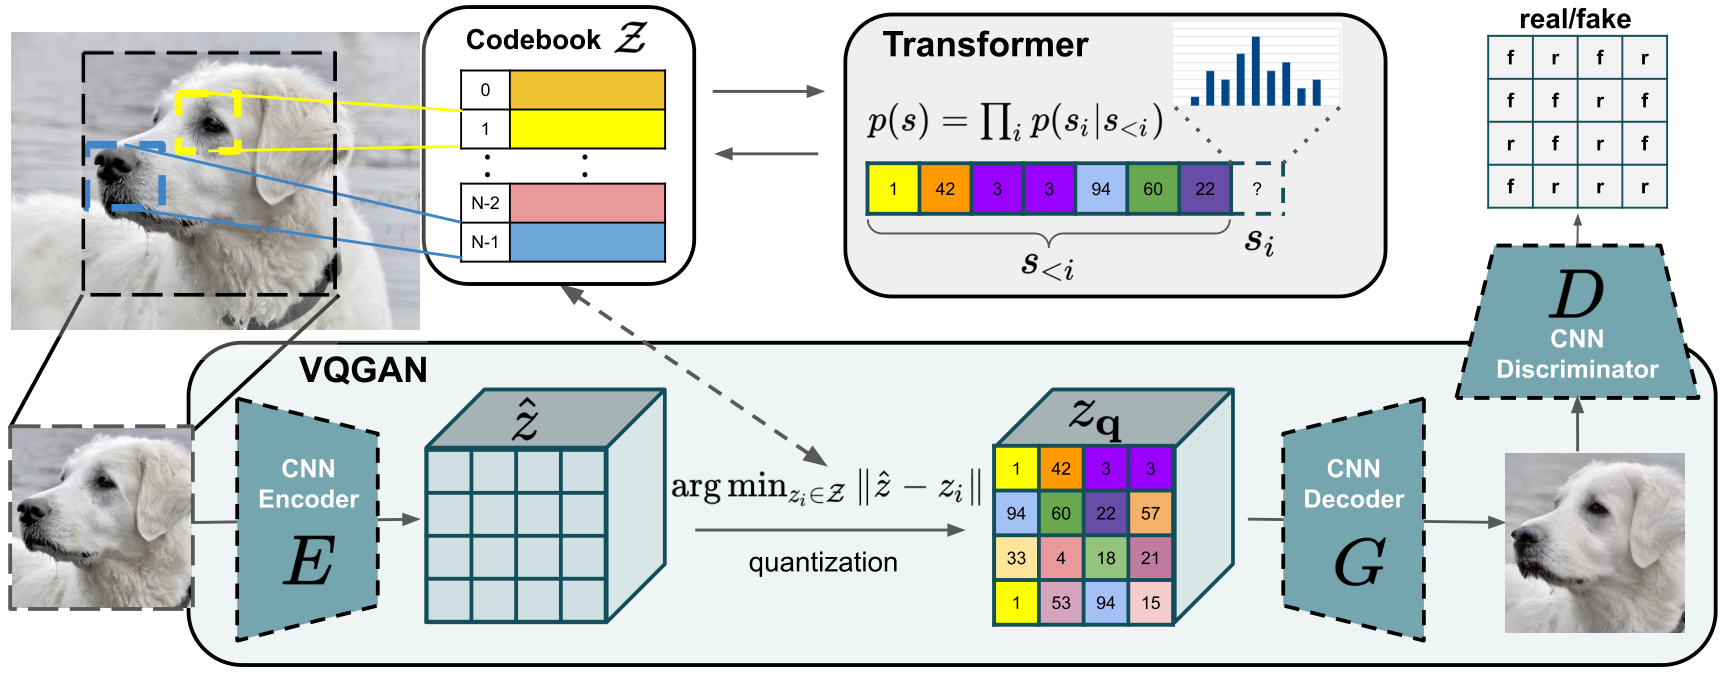
\includegraphics[width=0.9\linewidth]{concept_engineering/vqgan/vqgan.png}
    \caption{VQGAN visualization.\cite{Esser_2021_CVPR}. }
    \label{fig:vqgan-diagram}
\end{figure}

VQGAN is a hybrid model that combines VQVAE's structured latent space with GANs. VQGAN can create high-quality images by using GANs to make textures and details look more realistic.

\paragraph{Loss function}\mbox{}\\

The loss function for VQGAN combines VQVAE and GAN losses:

\begin{itemize}
    \item \textbf{VQVAE loss}: Reconstruction, Commitment and Codebook losses,
    \item \textbf{Adversarial Loss}: The GAN component introduces a discriminator that tries to distinguish between real and synthetic images, pushing the generator to create more realistic images.
    \item Perceptual similarity loss: ensures the generated image matches the real image in terms of higher-level features, most commonly LPIPS\footnote{\url{https://github.com/richzhang/PerceptualSimilarity}} is used for this puprpose.
\end{itemize}


the optimal compression target $Q^{\star}$ is expressed by VQVAE loss\eqref{loss_vq} and GAN loss\eqref{loss_gan} combined together in the formula
\begin{equation}
    Q^{\star} = \text{arg min}_{E,G,Z} \text{max}_D \mathbb{E}_{x~p(x)} [\underbrace{L_{VQ}(E, G, Z)}_{\text{VQVAE loss}} + \lambda\underbrace{L_{GAN}(N, D)}_{\text{adversarial loss}}],
\end{equation}

where $\lambda$ is the scaling factor.
% \begin{equation}
%     \mathcal{L}_{GAN}(N,D) = [\log D(x) + log(1-D(\hat{x}))]
% \end{equation}

% \paragraph{Training}\\
% VQGAN should be traon prostate CT scans, learning both a structured latent space and adversarial components to ensure realism.


\paragraph{Generation of CT scans}\mbox{}\\
\indent Generation of CT scans has the same procedure as VQVAE. Firstly LDM is trained and then output is passed through codebook, then decoder. 

% Train it on real CT scans
% To make a new scan, give it some random input
% It will use its codebook and GAN parts to make a realistic-looking CT scan
% % Loss function: VQGAN's loss has several components.

% To generate an artificial CT scan, train the VQGAN on prostate CT scans. This ensures realism.
% To generate a new scan, sample latent codes from the codebook and pass them through the GAN generator.

% To generate a new scan, sample discrete latent codes from the codebook and pass them through the GAN generator.
% The adversarial process refines the image to produce highly realistic synthetic CT scans with well-captured anatomical details.